\input{../../common/latex_asst_template/asst_template.tex}

\class{ECEN 625}
\term{Winter 2021}
\assttitle{Assignment 1: Graphs}
\duedate{Tuesday, January 15, 2019 11:59pm}


\setuppage

\begin{document}

\maketitle
\thispagestyle{fancy}

\section{Learning Outcomes}
The goals of this assignment are to:
\begin{itemize}
	\item Familiarize yourself with graph algorithms that are most applicable to HLS techniques, namely topological sorting and identifying the critical path.
	\item Observe the structure of commercial HLS data flow graphs.
	\item Practice C++ skills.
\end{itemize}

\section{Preliminary}
This assignent is located in the \texttt{asst\_graphs} folder.  All commands shown assume you are located in that folder in your terminal.

\subsection{Install Packages}
You will need the following packages:
\begin{lstlisting}
	sudo apt install cmake graphviz
\end{lstlisting}

\subsection{Extract Graphs}
Due to size contraints on Github, the graphs are in a zip files and need to be extracted.  Run the following to extract the graphs:
\begin{lstlisting}
	make unzip_graphs
\end{lstlisting}

\subsection{Inspect the code}
\begin{itemize}
	\item {\tt niGraphs/} -- This folder contains 2333 graphs of customer designs from National Instrument's HLS tool (LabVIEW Communications System Design Suite -- \url{http://www.ni.com/labview-communications/}).  Feel free to look at these files.  You will see each file defines a set of nodes and edges with associated properties.  As we progress through the class material you will learn more about these properties, but you can ignore most of them for now, aside from a few that are specifically mentioned in this assignment.
	\item {\tt src/niGraphReader/} -- This contains the NIGraphReader class, which will parse the graph files into NIGraph* data structures.
	\item {\tt src/niGraph/} -- This contains the NIGraph class, as well as NIGraphNode and NIGraphEdge classes, which are the data structures for the graphs.
	\item {\tt src/main.cpp} -- You will need to implement several functions in this file.  You are free to split your code into additional files if you desire.
\end{itemize}

\subsection{Build the code}
The project uses {\tt cmake} as a build manager.  {\tt cmake} is a tool that will automatically create necessary makefiles for use with the {\tt make} tool.
The code can be built using the following commands:
\begin{lstlisting}
cd build
cmake ../src
make
\end{lstlisting}

This will produce an executable located in \texttt{build/main}.  If you change any file contents, you only need to re-run \texttt{make} to recompile.  If you add new files, you will need to edit the \texttt{src/CMakeLists.txt} file.	



\section{Requirements}

\begin{figure}[p]
	\centering
		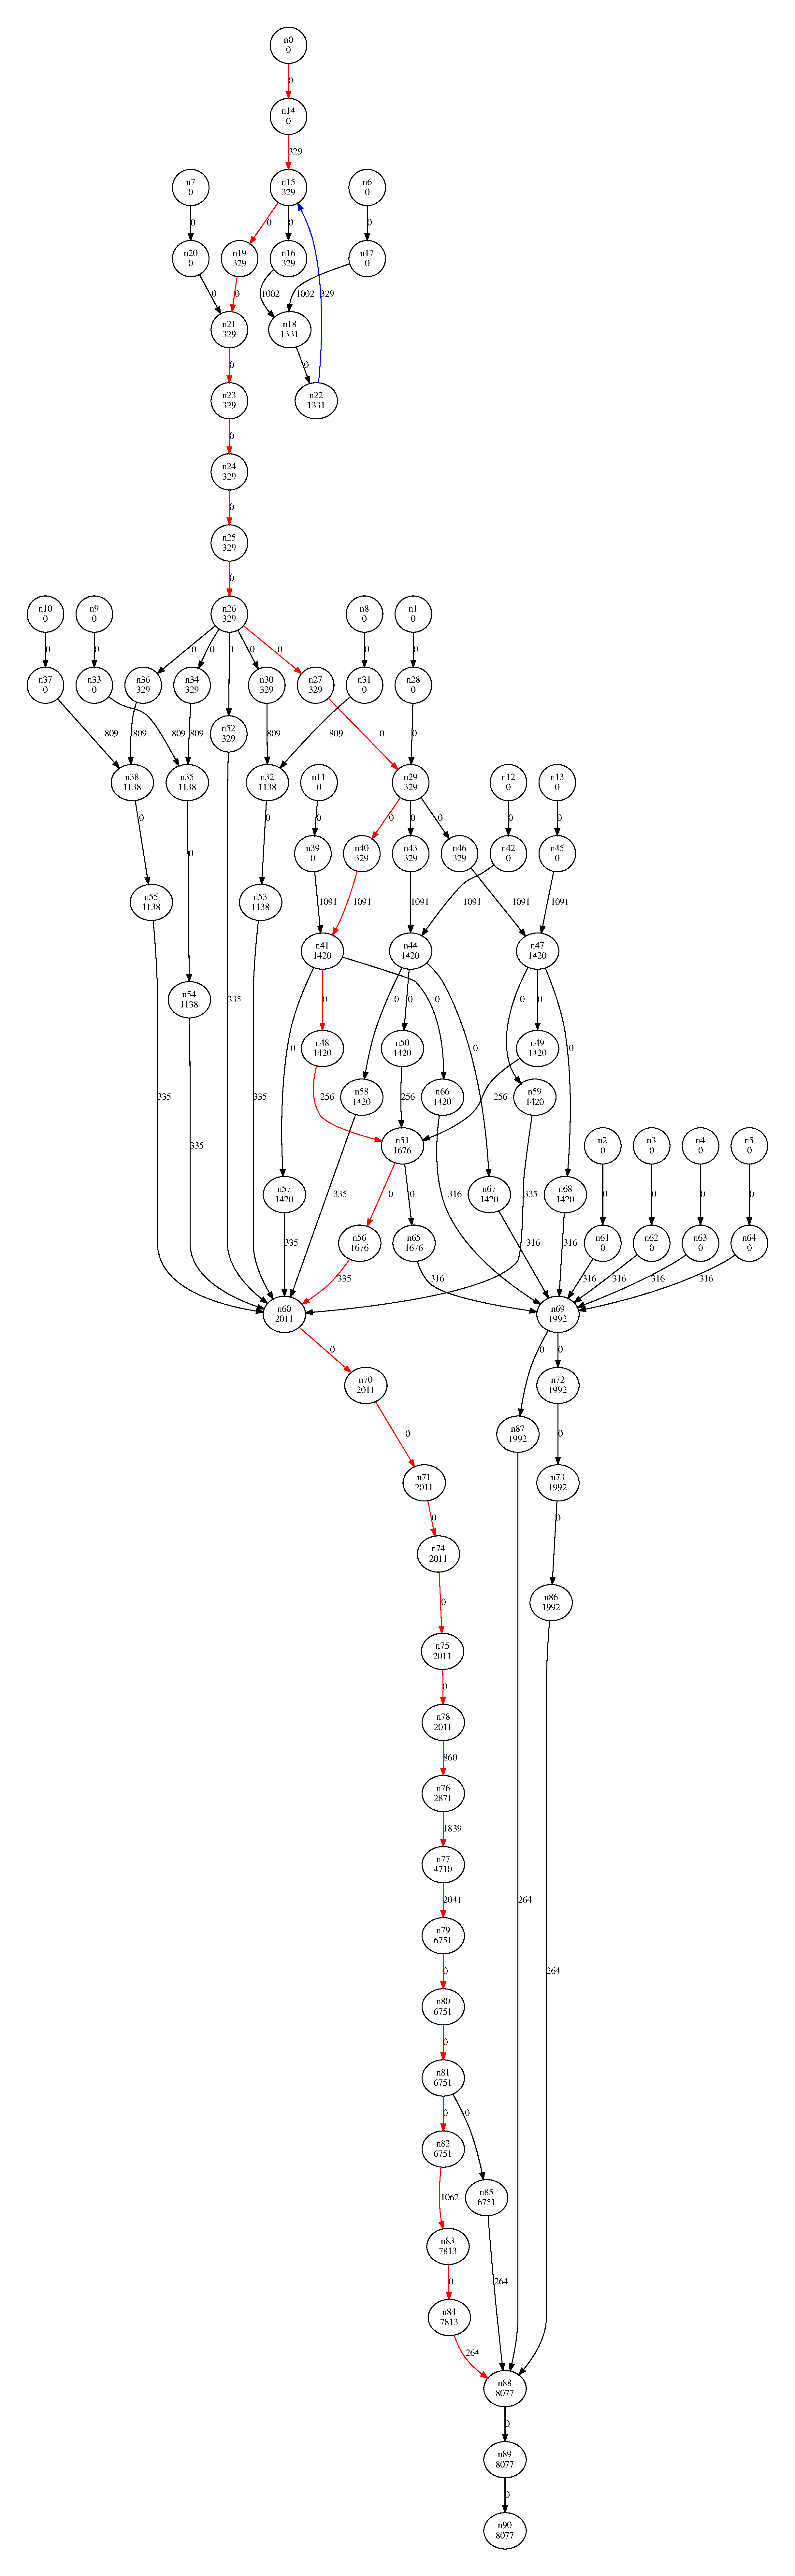
\includegraphics[width=\textwidth,height=.9\textheight,keepaspectratio]{graph0.pdf}
	\caption{DelayGraph\_0}
	\label{fig:graph0}
\end{figure}

The goal of this lab is to perform a topological sort of a dataflow graph, identify the longest delay path, and create a graph visualization.  \cref{fig:graph0} shows a the graph for \texttt{DelayGraph\_0.graphml}. 
Your graphs should have the following properties:
\begin{itemize}
	\item Show all nodes and edges. Some nodes don't have edges.
	\item Nodes should be labeled with the node {\tt id}, and the longest delay path to reach the node.
	\item Edges should be labeled with the edge {\tt delay}.
	\item Edges along the longest delay path (ie, the critical path), should be colored red.
	\item The provided graphs are \textbf{textit{almost}} directed acyclic graphs (DAGs), except for a few \textit{feedback edges}, which create cycles.  These feedback edges should be colored in blue.
\end{itemize}

\subsection{\texttt{main()}}

The provided main function can be run in two modes:

\begin{description}
	\item[Mode 1: Selective graphs] You can provide a list of graph numbers as arguments to main: 
	\begin{lstlisting}
		./main 1 7 1300
	\end{lstlisting}
	For each graph this will perform topological sorting and print the sorted list of nodes, find the longest path, and generate a DOT file and PDF.  Statistics are printed to a \texttt{results.txt} file.
	\item[Mode 2: All graphs] If you provide no arguments, all graphs will be processed.  The sorted graph nodes won't be printed, and no DOT files will be generated.
\end{description}


\subsection{Part 1: Visualizing Graphs}
\label{sec:del1}

You must write code to output an {\tt NIGraph} structure in DOT language.  The code should be added to the following function:

\begin{lstlisting}
void createDOT(const NIGraph &graph, const std::string outputPath,
    NIGraphNodeList &longestPath,
    std::map<NIGraphNode *, int> &nodeDelays) {
  
}
\end{lstlisting}

See \url{http://www.graphviz.org/content/dot-language} for the specification of the DOT language.  For example, a simple DAG with two nodes ({\tt a} and {\tt b}) and one edge ({\tt delay} = 3) may have a DOT file like this:

\begin{lstlisting}
strict digraph {
  a [label="a\n0"];
  b [label="b\n3"];
  a -> b [label=3; color=red];  
}
\end{lstlisting}

Although the graph visualization relies on the longest path data, it is included first in this document as visualizing the graphs can sometimes be helpful in debugging your sorting or longest path analysis code.  So, I suggest you complete the graph visualization without the longest path data first, then return and finish this step once you have the longest path analysis working.


\subsection{Part 2: Topological Sorting}
\label{sec:del2}
You will write code to perform a topological sort of a graph.  See lecture slides or \url{https://en.wikipedia.org/wiki/Topological_sorting}.


The code should be added here:
\begin{lstlisting}
NIGraphNodeList topologicalSort(const NIGraph &graph) {
  NIGraphNodeList q; 
  // add code here	  
  return q;
}
\end{lstlisting}
The function has a single input, an {\tt NIGraph}, and returns a topologically sorted list of nodes ({\tt NIGraphNode*}).  Topological order is such that for every directed edge $uv$ from node $u$ to node $v$, $u$ comes before $v$ in the ordering.  Since a topological sort is only possible for directed acyclic graphs (DAGs), you will need to \uline{ignore the feedback edges}.  

\subsection{Part 3: Longest Path}
\label{sec:del3}
In this last section you will write code to find the longest delay path in the graph, using the topologically sorted nodes from Part 2.  This code should be written in this function:
\begin{lstlisting}
int longestDelayPath(const NIGraphNodeList &topolSortedNodes,
    NIGraphNodeList &longestPath,
    std::map<NIGraphNode *, int> &nodeDelays) {
  // add code here
}
\end{lstlisting}
The first arugment to this function is the topologically sorted list of nodes in the graph.  The function populates two data structures: \texttt{longestPath} should be populated with a list of nodes that make up the longest path, from start to finish, and \texttt{nodeDelays} provides a map indicating the longest delay to each node in the graph.  The delay of the longest path is returned from the function.

See lecture slides, \url{https://en.wikipedia.org/wiki/Longest_path_problem}, or search on the web for how to determine the longest path from a topological sort. For a DAG, the longest delay path is also known as the \emph{critical path}.  This term is likely familiar to you in the circuit domain, as combinational logic can be represented using a DAG, and the critical path restricts the maximum frequency of the circuit.  

Again, to ensure the graph is a DAG, you will \uline{need to ignore feedback edges}. Remember to ignore these edges when finding the longest back, and during the backtracking portion.


\section{Deliverables}

\paragraph{Deliverables:} Choose any two graphs you like (aside from DelayGraph\_0) and include an image such as \cref{fig:graph0} in your report.  Make sure the graph isn't too large, or it won't be readable.  Anything much larger than the provided example is probably too large.  



\paragraph{Deliverables:} Write a short paragraph about how your topological sorting algorithm works.  

Include a scatter plot (\url{https://en.wikipedia.org/wiki/Scatter_plot}), which plots the run-time for your topological sort code for {\bf ALL} 2333 of the provided graphs.  The plot should be of the following format:



\begin{itemize}
	\item The x-axis should show the size of the graph ($V + E$)
	\item The y-axis should show the runtime of the topological sorting.
	\item Both the x and y axis should be in logarithmic scale, with appropriate ranges to fit your data points.
\end{itemize}

There are many ways to do a topological sort.  For full marks, your chart data should show that your algorithm complexity is approximately $O(V+E)$.  Please don't spend extra time performing analysis to show this -- just a visual inspection of the scatter plot is fine.


\paragraph{Deliverables:}
Include the following data using your longest path code:
\begin{itemize}
	\item Include the following table in your report, with all values populated:
	\begin{table}[h!]
	\centering
	\begin{tabular}{|l|r|r|} \hline
	{\bf Graph} & {\bf size ($V+E$)} & Delay \\ \hline
	DelayGraph\_0 & 197 & 8077 \\ \hline
	DelayGraph\_1 &  &  \\ \hline
	DelayGraph\_2 &  &  \\ \hline
	DelayGraph\_3 &  &  \\ \hline
	DelayGraph\_4 &  &  \\ \hline
	DelayGraph\_5 &  &  \\ \hline
	DelayGraph\_6 &  &  \\ \hline
	DelayGraph\_7 &  &  \\ \hline
	DelayGraph\_8 &  &  \\ \hline
	DelayGraph\_9 &  &  \\ \hline
	DelayGraph\_10 &  &  \\ \hline

	\end{tabular}
	\end{table}
	
	\item Include the longest path for DelayGraph\_3.  
	
	For example, the longest path for DelayGraph\_0 is:
	\begin{lstlisting}
n0 -> n14 -> n15 -> n19 -> n21 -> n23 -> n24 -> n25 -> n26 -> n27 -> 
n29 -> n43 -> n44 -> n50 -> n51 -> n56 -> n60 -> n70 -> n71 -> n74 -> 
n75 -> n78 -> n76 -> n77 -> n79 -> n80 -> n81 -> n82 -> n83 -> n84 -> 
n88

	\end{lstlisting}
\end{itemize}

\section{Coding Guidelines}
\begin{itemize}
	\item Your code should be added to the {\tt src/522r\_asst1.cpp} file.  You can add additional files if you like, just don't forget to submit them.  You shouldn't change the {\tt niGraph*} files.
  \item You are free to add extra helper functions, but you should not change the definition of the provided functions. 
	%\item All graph objects ({\tt NIGraph}, {\tt NIGraphNode}, {\tt NIGraphEdge}) should be allocated by the {\tt parseGraphMlFile()} function.  Do not allocate these objects yourself.  Example object allocations, which you should not do:
	%\begin{lstlisting}
	%NIGraphNode * node1 = new NIGraphNode();
	%NIGraphNode node2;
	%\end{lstlisting}
	\item I have made {\tt topologicalSort()} return a  {\tt std::deque} instead of a {\tt std::vector}, as it supports $O(1)$ insertion at the front or back of the list ({\tt std::vector} is $O(n)$ insertion at the front).  Since different topological sorting algorithms require inserting at the front or back, I wanted to provide this functionality.
	%\item Topological order is such that for every directed edge $uv$ from vertex $u$ to vertex $v$, $u$ comes before $v$ in the ordering.  For the output of {\tt topologicalSort()}, and the input to {\tt longestDelayPathFromTopolSortedNodes()} you are free to use topological or reverse topological ordering.  When I implemented the code, the topological sorting algorithm I used added items to the vector in reverse topological order.  To avoid inserting at the start of the vector, which is $O(n)$, I just inserted items at the end of the vector, which is $O(1)$, and returned the reverse topological ordering.  You should choose the appropriate ordering for the algorithm you use.  (An alternative would be to use a data structure that supported $O(1)$ insertion at the front, such as {\tt std::deque}; however, for simplicity I chose to define the function as returning a {\tt std::vector}).
	\item It doesn't matter what code you submit in {\tt main()}, you will only be marked on the code in the required functions, and any code that those functions call.
\end{itemize}

\section{Submission Instructions}

\begin{enumerate}
	\item 

Submit a report containing the following items:
\begin{itemize}
	\item Your name :)
	\item The two DOT graph images, described in \cref{sec:del1}.
	\item The paragraph describing your algorithm, and scatter plot, from \cref{sec:del2}.
	\item The table, and longest path, described in \cref{sec:del3}.
	\item Feedback about the assignment
	
	\begin{itemize}
		\item How many hours you spent on the assignment?  
		\item How challenging was the C++ coding?
		\item Anything you liked?
		\item Anything you didn't like? Or anything you would change?
		\item Did you find the assignment worthwhile? Why or why not?
	\end{itemize}
\end{itemize}

\item Submit your source code.  If you only change the one .cpp file, then only submit that file.
\end{enumerate}


\textbf{Send your report and code to \href{mailto:jgoeders@byu.edu}{jgoeders@byu.edu} with the subject: 625 Asst1}

\section{Evaluation Criteria}
The three deliverables will be weighted equally.  You will be marked based on completion, adherence to specification, correctness of code, efficiency of code, and readability of code.




\end{document}
